\documentclass{sigchi}

% Use this command to override the default ACM copyright statement
% (e.g. for preprints).  Consult the conference website for the
% camera-ready copyright statement.

%% EXAMPLE BEGIN -- HOW TO OVERRIDE THE DEFAULT COPYRIGHT STRIP -- (July 22, 2013 - Paul Baumann)
% \toappear{Permission to make digital or hard copies of all or part of this work for personal or classroom use is      granted without fee provided that copies are not made or distributed for profit or commercial advantage and that copies bear this notice and the full citation on the first page. Copyrights for components of this work owned by others than ACM must be honored. Abstracting with credit is permitted. To copy otherwise, or republish, to post on servers or to redistribute to lists, requires prior specific permission and/or a fee. Request permissions from permissions@acm.org. \\
% {\emph{CHI'14}}, April 26--May 1, 2014, Toronto, Canada. \\
% Copyright \copyright~2014 ACM ISBN/14/04...\$15.00. \\
% DOI string from ACM form confirmation}
%% EXAMPLE END -- HOW TO OVERRIDE THE DEFAULT COPYRIGHT STRIP -- (July 22, 2013 - Paul Baumann)
\toappear{}

% Arabic page numbers for submission.  Remove this line to eliminate
% page numbers for the camera ready copy
% \pagenumbering{arabic}

% Load basic packages
\usepackage{balance}  % to better equalize the last page
\usepackage{graphics} % for EPS, load graphicx instead 
\usepackage[T1]{fontenc}
\usepackage{txfonts}
\usepackage{mathptmx}
\usepackage[pdftex]{hyperref}
\usepackage{color}
\usepackage{booktabs}
\usepackage{textcomp}
% Some optional stuff you might like/need.
\usepackage{microtype} % Improved Tracking and Kerning
% \usepackage[all]{hypcap}  % Fixes bug in hyperref caption linking
\usepackage{ccicons}  % Cite your images correctly!
% \usepackage[utf8]{inputenc} % for a UTF8 editor only

% If you want to use todo notes, marginpars etc. during creation of your draft document, you
% have to enable the "chi_draft" option for the document class. To do this, change the very first
% line to: "\documentclass[chi_draft]{sigchi}". You can then place todo notes by using the "\todo{...}"
% command. Make sure to disable the draft option again before submitting your final document.
\usepackage{todonotes}
\usepackage[frenchb]{babel}
%\frenchbsetup{og = �, fg = �}

% Paper metadata (use plain text, for PDF inclusion and later
% re-using, if desired).  Use \emtpyauthor when submitting for review
% so you remain anonymous.

%----------------------------------------------------------------------------------------
% Title, Authors, Keywords
%----------------------------------------------------------------------------------------
\def\plaintitle{Reachability of the Thumb on Portable Tangible Sliders}
\def\plainauthor{First Author, Second Author, Third Author,
  Fourth Author, Fifth Author, Sixth Author}
\def\emptyauthor{}
\def\englishkeywords{Authors' choice; of terms; separated; by
  semicolons; include commas, within terms only; required.}
\def\frenchkeywords{Format ; instructions ; qualit\'{e} ; actes de conf\'{e}rence ; les mots cl\'{e}s doivent \^{e}tre s\'{e}par\'{e}s par des point-virgules.}
\def\plaingeneralterms{Documentation, Standardization}
%----------------------------------------------------------------------------------------

% llt: Define a global style for URLs, rather that the default one
\makeatletter
\def\url@leostyle{%
  \@ifundefined{selectfont}{
    \def\UrlFont{\sf}
  }{
    \def\UrlFont{\small\bf\ttfamily}
  }}
\makeatother
\urlstyle{leo}

% To make various LaTeX processors do the right thing with page size.
\def\pprw{8.5in}
\def\pprh{11in}
\special{papersize=\pprw,\pprh}
\setlength{\paperwidth}{\pprw}
\setlength{\paperheight}{\pprh}
\setlength{\pdfpagewidth}{\pprw}
\setlength{\pdfpageheight}{\pprh}

% Make sure hyperref comes last of your loaded packages, to give it a
% fighting chance of not being over-written, since its job is to
% redefine many LaTeX commands.
\definecolor{linkColor}{RGB}{6,125,233}
\hypersetup{%
  pdftitle={\plaintitle},
% Use \plainauthor for final version.
%  pdfauthor={\plainauthor},
  pdfauthor={\emptyauthor},
  pdfkeywords={\englishkeywords},
  bookmarksnumbered,
  pdfstartview={FitH},
  colorlinks,
  citecolor=black,
  filecolor=black,
  linkcolor=black,
  urlcolor=linkColor,
  breaklinks=true,
}

% create a shortcut to typeset table headings
% \newcommand\tabhead[1]{\small\textbf{#1}}

% End of preamble. Here it comes the document.
%----------------------------------------------------------------------------------------
\begin{document}

\title{\plaintitle}

\numberofauthors{3}
\author{%
  \alignauthor{Premier Auteur\\
    \affaddr{Affiliation}\\
    \affaddr{Code postal, Ville, Pays}\\
    \email{Adresse email}}\\
  \alignauthor{Deuxi\`{e}me Auteur\\
    \affaddr{Affiliation}\\
    \affaddr{Code postal, Ville, Pays}\\
    \email{Adresse email}}\\
  \alignauthor{Troisi\`{e}me Auteur\\
    \affaddr{Affiliation}\\
    \affaddr{Code postal, Ville, Pays}\\
    \email{Adresse email}}\\
}

%================================================
%\begin{figure*}[h]
%  \centering
%  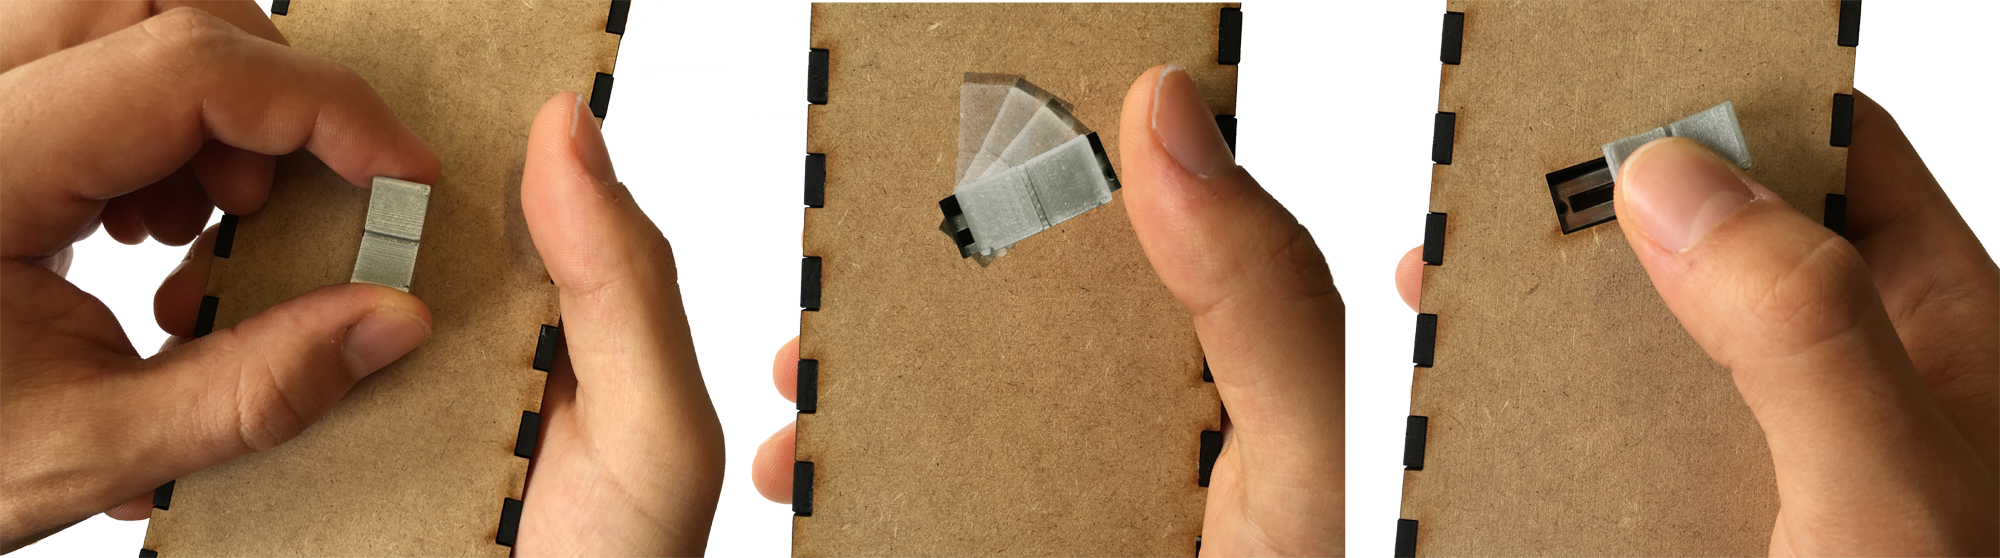
\includegraphics[width=1.7\columnwidth]{figures/portada}
%  \caption{GraspMe concept: the slider changes size and orientation according to the way how it is operated}
%\end{figure*}
%================================================ 

\maketitle


%----------------------------------------------------------------------------------------
\begin{resume} % R�sum�
%----------------------------------------------------------------------------------------
	MAJ---\today. Cet article d\'{e}crit et utilise le format de mise en page \`{a} respecter pour les soumissions \`{a} IHM'16. Apr\`{e}s acceptation, ces soumissions seront publi\'{e}es dans les actes d'IHM'16, ainsi que sur l'ACM Digital Library, sauf les communications informelles qui seront publi\'{e}es dans un volume annexe s\'{e}par\'{e}. Comme certains \'el\'ements ont chang\'{e} par rapport aux ann\'{e}es pr\'{e}c\'{e}dentes, nous vous prions de bien lire ce document m\^{e}me si vous avez d\'{e}j\`{a} soumis \`{a} IHM auparavant.
	  
  Le format d\'{e}crit dans ce document doit \^{e}tre respect\'{e} pour les soumissions \`{a} la conf\'{e}rence IHM. Nous souhaitons faire des actes d'IHM un document de qualit\'{e} \`{a} la pr\'{e}sentation homog\`{e}ne. Nous demandons donc aux auteurs de respecter quelques r\`{e}gles simples. 
  
  Nous vous demandons principalement de faire en sorte que votre article ressemble exactement \`{a} ce document. La meilleure fa\c{c}on d'y parvenir est de t\'{e}l\'{e}charger l'un des mod\`{e}les propos\'{e}s depuis le site web de la conf\'{e}rence IHM, \url{http://ihm16.afihm.org/#!contribution}, et de remplacer son contenu par le v\^otre.
\end{resume}

\motscles{\frenchkeywords} %Mots cl�s
%----------------------------------------------------------------------------------------

%----------------------------------------------------------------------------------------
\begin{abstract} % English Abstract (mandatory)
%----------------------------------------------------------------------------------------
  UPDATED---\today. This article describes the formatting requirements for IHM'16. After acceptance, these submissions will be published in the proceedings of IHM'16 and the ACM Digital Library. As some items have changed from previous years, please read the document carefully, even if you have submitted to IHM before. Please add an additional abstract in English, along with the French version.
\end{abstract}

\keywords{\englishkeywords} % English keywords (mandatory)
%----------------------------------------------------------------------------------------

%----------------------------------------------------------------------------------------
\category{H.5.m.}{Information Interfaces and Presentation
  (e.g. HCI)}{Miscellaneous} \category{See
  \url{http://acm.org/about/class/1998/} for the full list of ACM
  classifiers. This section is required.}{}{}
%----------------------------------------------------------------------------------------

%----------------------------------------------------------------------------------------
\section{Introduction}
%----------------------------------------------------------------------------------------
Current portable devices let us interact with applications or appliances in a discrete or continuous manner. Digital sliders have been used to control a wide diversity of functions (e.g. a device’s screen brightness or volume) and appliances such as mixing consoles and smart house’s control panel at distance. Though digital sliders offer flexibility of arrangement in the screen, a key feature is lost with graphical widgets that can be achieved with tangible sliders, such as eyes-free interaction.

The benefits of tangible elements are well known in the HCI community. For instance in \cite{Jansen:2012:TRC:2207676.2208691} Jansen et al. presented tangible sliders, which could be placed on top of a tablet’s screen, were used to control wall-size displays. The benefits of the tangible and mobile interaction let participants of the study control an object at distance while carrying the portable device and being eyes-free from the device. The usefulness of merging sliders and tangibility for mobile and distant interaction was also examined in \cite{unpublished}. In this study, authors showed that even when the location was changed by the system, a tangible slider was more accurate than a graphical slider. In this work we will also focus on deformable tangible interfaces, particularly on tangible sliders, for mobile interaction. We aim at further informing the system-driven design of tangible sliders on mobile devices. 

An important factor for placing tangible sliders on mobile devices is the number of users’ hands available for interaction. 45\% of users state they use one hand for almost all mobile interactions and only 19\% stated the same for two hands \cite{Karlson06}. 66\% of users state they would prefer using just one hand for the tasks and only 9\% would prefer using both hands \cite{Karlson06}. An observational study \cite{hoober13} showed that from 780 persons there are three basic ways in which users hold their mobile phones while interacting with it: 49\% interacted with the same hand that holds the phone, 36\% interacted with one hand while holding the device with the other hand and 15\% interacted with both hands. 

This preference of one-hand interaction brings a challenge related to interaction with handheld touchscreen: the incapacity of users to reach the entire surface with the thumb of the hand that holds the device. The area that can be reached with the thumb is called functional area of the thumb (Figure \ref{fig:figure1}) and designers have long been aware of this problem. Several heuristics estimates of the functional area of the thumb have been proposed \cite{hoober13,Clark,Curtis,Wroblewski} to serve as reference and a model to estimate the functional area of the thumb was presented in \cite{Bergstrom-Lehtovirta:2014:MFA:2611528.2557354}.

%================================================
\begin{figure}[h]
\centering
  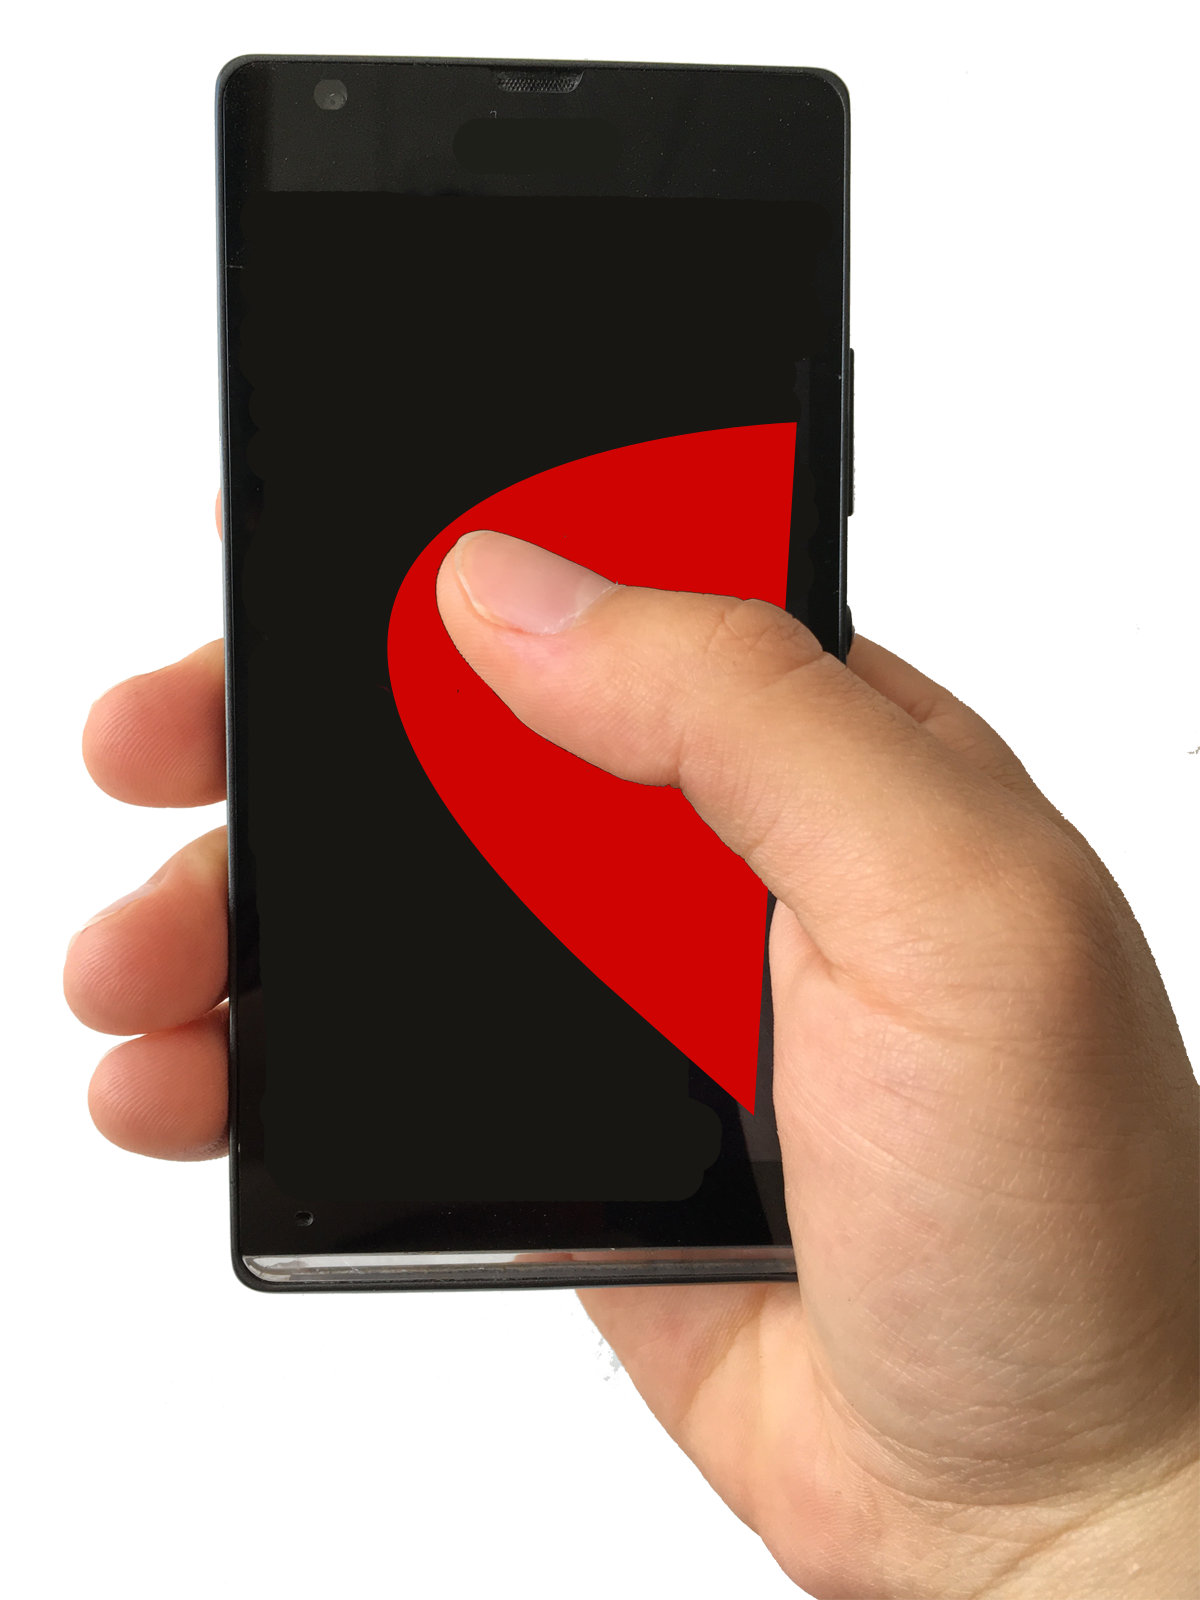
\includegraphics[scale=0.15]{figures/functAreaThumb}
  \caption{An estimation of the easy difficulty level of the functional area of the thumb (in red) on a mobile phone}
  \label{fig:figure1}
\end{figure}
%================================================

Despite the studies on the reachability of the thumb, some manufacturers keep using design guidelines that do not take into account the functional area of the thumb. 
For instance Apple’s interface guidelines for mobile devices suggest that “Back” and “Action” buttons on the top-right and left corners; while the “Tab” bar should be placed at the bottom of the screen. To reach such elements people tend to tilt or shift the device in the hand. This change of grip has been observed in several studies \cite{Karlson06understandingsingle-handed,Goel:2012:GUB:2380116.2380184,Negulescu:2015:GCI:2702123.2702185}, and might counterbalance the reachability problem for some area of mobile devices. 

Shape-changing mobile devices brings new elements (physical objects) on top of the flat screen surface. It is not clear if this will further increase the need to change the grip or the ability to operate the slider within the functional area of the thumb. In this paper, we study the impact on performance and grip of the design of a tangible slider on a mobile device.

We conducted an experiment to originally study the impact of the grip of the device, when operated with one-hand and with two-hands, on performance; aiming to motivate a deformable tangible slider. The results showed that one slider type outperformed the rest for both one-hand and two-hands interaction. For this reason we focused our results to analyse the effect of operating tangible sliders within the easy and medium difficulty levels of the functional area of the thumb and thus, considering the grip changing effect.

We built four prototypes in which we tested four different conditions: large-vertical, large-tilted, small-vertical and small-tilted sliders; being the large-vertical the only condition going out of the easy level of the functional area of the thumb. Participants performed a pointing task by holding each prototype with one and two hands. Results showed a marginal statistically significant difference between the two large sliders (vertical and tilted) and a considerable significant difference between the small and the large sliders for one-hand operation. This lead us to conclude that:

\begin{enumerate}
\item Regardless of the difficulty level of the functional area of the thumb it is the motor space, which impacts significantly the performance
\item The small shift of the hand grip required between the easy and medium difficulty level does not impact on the performance
\end{enumerate}

%----------------------------------------------------------------------------------------
\section{Related Work}
%----------------------------------------------------------------------------------------
Nowadays touch interaction is almost omnipresent on mobile devices and technological advances have made screens bigger. The users can then interact with more content displayed on screen but it is more difficult for the users to reach with one thumb all the parts of the screen.

%----------------------------------------------------------------------------------------
\subsection{Studying the functional area of the thumb}
%----------------------------------------------------------------------------------------
The commonly used touch interaction on mobile devices motivated several studies on the functional area in which our thumbs can easily operate. Heuristic approximations of the functional area of the thumb \cite{hoober13,Clark,Curtis,Wroblewski} have been proposed to give designers insights about the reachable area of the interface when mobile devices are operated with the thumb. In \cite{Karlson06understandingsingle-handed} an empirical study demonstrated that areas difficult to reach for thumb interaction (common in large mobile devices) provoke a significant slowdown (between 7\% and 12\%) in movement time; they also showed that users perceive the difficulty of reaching areas with the thumb between easy, medium and hard; and showed that some thumb’s movements (Figure \ref{fig:figure6}a) are more complex than others (Figure \ref{fig:figure6}b). In \cite{Bergstrom-Lehtovirta:2014:MFA:2611528.2557354}, Bergstrom-Lehtovirta \& Oulasvirta proposed a model to estimate the functional area of the thumb, by giving grip related information (surface size, hand size, and position of the index finger on the back of the device), is presented; the model gives as a result the functional area that is commonly an area under a parabolic curve. These studies put in evidence that performance can decrease as screens get larger, as a consequence of bigger areas outside the functional area of the thumb.

%----------------------------------------------------------------------------------------
\subsection{Dealing with out-of-reach elements on the interface}
%----------------------------------------------------------------------------------------
Motivated by the fact that some screen areas are difficult to reach with the thumb, researchers have proposed several technical solutions. In \cite{Karlson:2007:TGO:1776994.1777034}, Karlson \& Bederson presented a technique that generates a proxy view of the whole interface and display it within the functional area of the thumb. In \cite{Roudaut:2008:TMI:1385569.1385594} Roudaut et al. presented a “magnetized” cursor can be manipulated through a telescopic stick which the user controls with the thumb’s movement. In \cite{Yu:2013:RSH:2493190.2493202} Yu et al. presented two techniques to assist users accessing out of reach elements for one-hand operation by determining the functional area of the thumb and mapping the gestures done inside the functional area with the whole interface. Authors also conducted a pilot study, which revealed that users prefer direct-touch over the techniques proposed in \cite{Karlson:2007:TGO:1776994.1777034,Roudaut:2008:TMI:1385569.1385594}; regardless of advantages of the techniques, these were tried only for very difficult areas to reach with the thumb. Authors also noticed that some techniques became difficult to operate due to the continuous change of grip of the device (e.g. for the technique presented in \cite{Karlson:2007:TGO:1776994.1777034} if the user changes the grip then the functional area of the thumb changes and the one computed before the grip change becomes inefficient).

%================================================
\begin{figure}[h]
\centering
  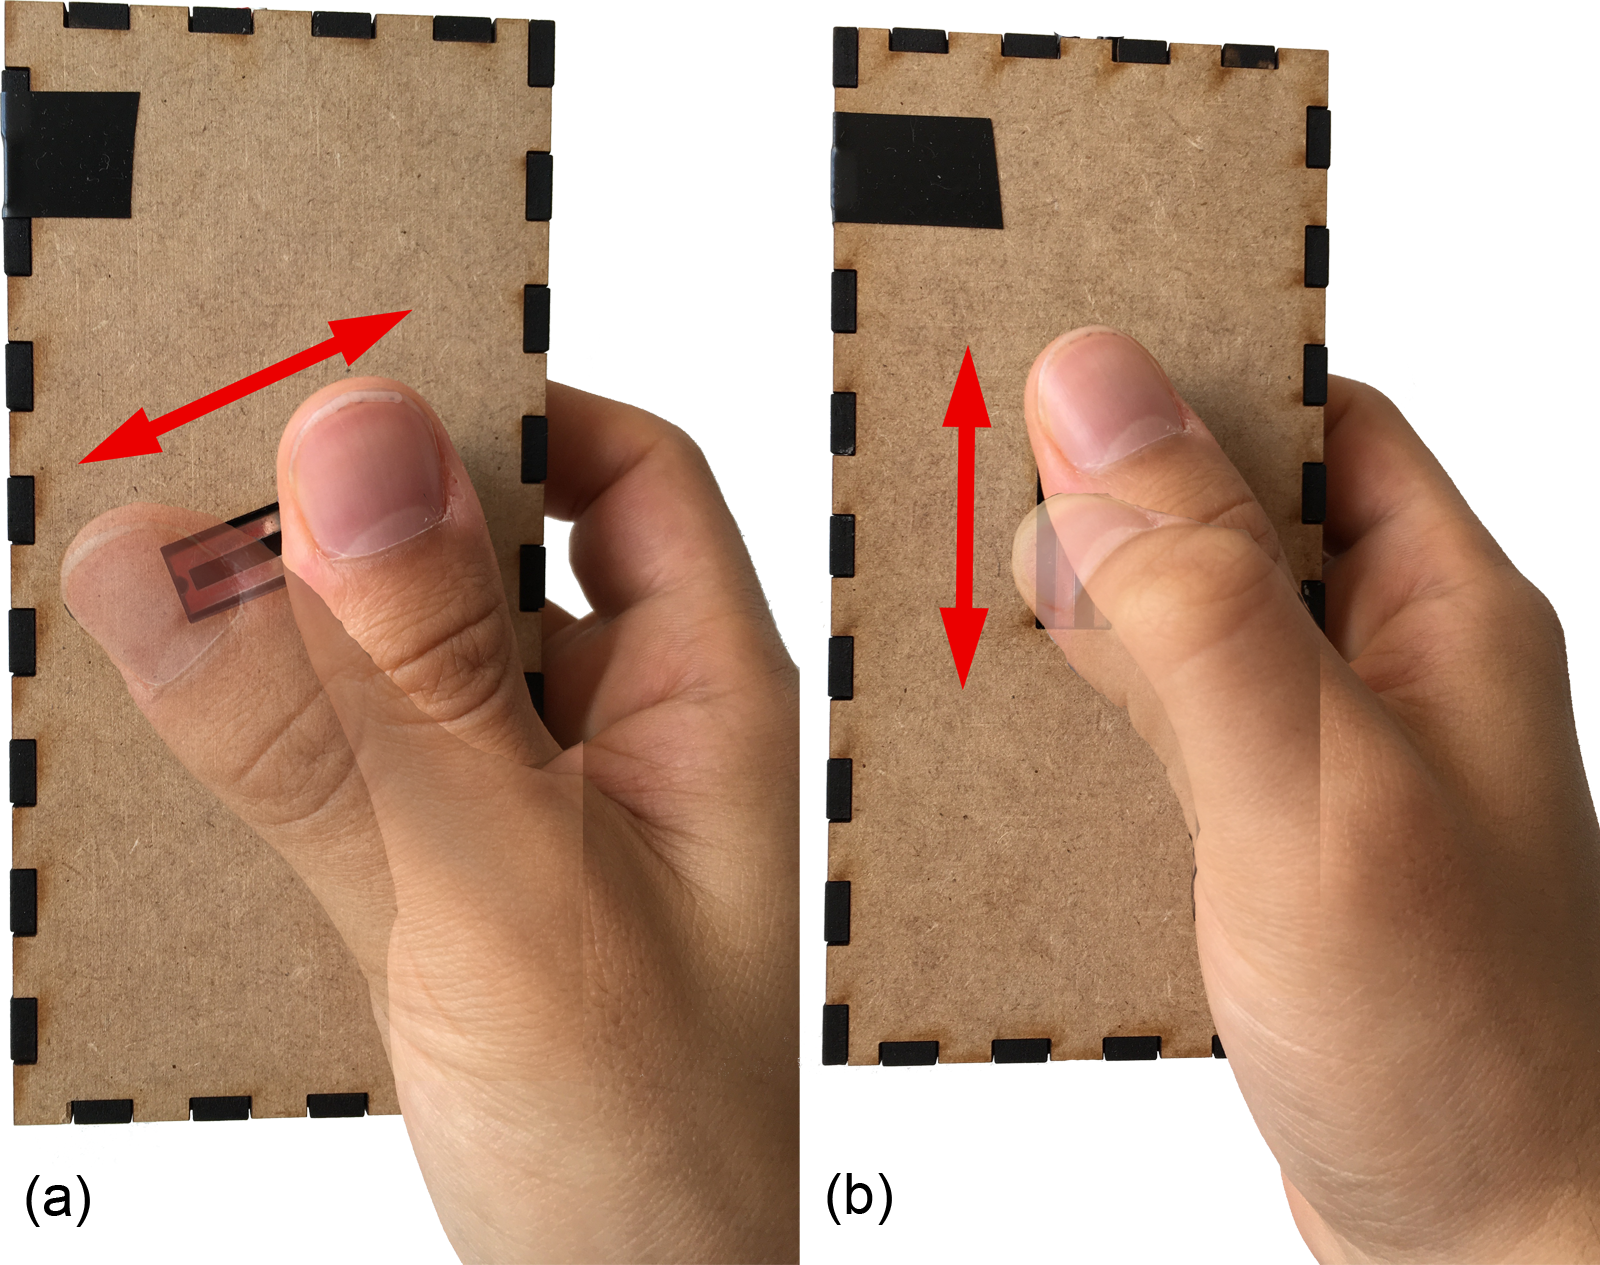
\includegraphics[width=1\columnwidth]{figures/thumbMove}
  \caption{(a) adduction-abduction movement of the thumb. (b) flexion-extension movement of the thumb}
  \label{fig:figure6}
\end{figure}
%================================================

%----------------------------------------------------------------------------------------
\subsection{A side effect in thumb interaction: grip change}
%----------------------------------------------------------------------------------------
Users tend to change their grip of the mobile device when reaching targets outside the functional area of the thumb, provoking a tilt or shift of the device inside the hand. This behavior is commonly seen in large portable devices: In \cite{Goel:2012:GUB:2380116.2380184} Goel et al. explored the rotation of the mobile device performed by the hand of the user when reaching areas outside the functional area of the thumb; authors used this information to propose a technique that identifies the hand posture in order to extend the awareness capabilities of mobile devices. This behavior is important to the point that in \cite{Karlson06understandingsingle-handed,Bergstrom-Lehtovirta:2014:MFA:2611528.2557354} participants of the experiments were restricted from spontaneously change the grip of the mobile device to avoid unexpected changes in the functional area of the thumb; in \cite{Negulescu:2015:GCI:2702123.2702185} Negulescu \& McGrenere presented a model that predicts the intended user’s touchdown (area in which the finger will land) when interacting with the device’s screen, by analyzing the changes (tilt and shift) of the grip of a mobile phone when the user tries the maximum reach of the current hand posture. In \cite{Hong:2013:TVC:2468356.2468589} Hong \& Lee proposed a software solution through a graphical control which the user can invoke to access key functions and thus help with the stability of the grip on the mobile devices and avoid unsafe grip changes.

So far all the work related to the functional area of the thumb has been done for graphic user interfaces on portable devices. In this work we will focus the functional area of the thumb for tangible interfaces as this brings new elements (physical objects) on top of the flat screen surface, particularly we will explore the impact of performing a pointing task within the easy and medium difficulty levels of the functional area of the thumb with tangible sliders on a mobile device operated with one hand.

So far all the work related to the functional area of the thumb has been done for graphical user interfaces. As the benefits of tangibility were demonstrated for mobile devices \cite{Jansen:2012:TRC:2207676.2208691}, even in the case of shape-changing mobile TUI \cite{unpublished}, in this work we focus on the functional area of the thumb for tangible interfaces. This brings new challenges through the new elements (physical objects) on top of the flat screen surface. Particularly we will explore the impact of performing a pointing task within the easy and medium difficulty levels of the functional area of the thumb with tangible sliders on a mobile device operated with one hand.

%----------------------------------------------------------------------------------------
\section{Experiment}
%----------------------------------------------------------------------------------------
We conducted an experiment to originally evaluate the impact on pointing performance and grip of the size and orientation of a tangible slider on a mobile device, aiming for a deformable slider. Due to the results given, we changed our focus to analyse the effect of operating tangible sliders within the easy and medium difficulty levels of the functional area of the thumb and thus, considering the grip changing effect. The experiment followed a within-subjects design with three independent variables:

\begin{itemize}
\item \textbf{Length:} Small, large
\item \textbf{Orientation:} Vertical, tilted
\item \textbf{Number of Hands (NH):} One- or two-handed
\end{itemize}

The Length variable refers to the travel length of the slider’s knob, the values are: 20mm length and 70mm length. The Orientation variable is composed of two states: vertical (90 degrees) and tilted (68 degrees). Commercial sliders widgets vary in length from 20mm to 100mm \cite{Coutrix2015}; in \cite{Hirotaka:2003:RCC:765891.766081} the movement range of the thumb was analysed and authors stated an average thumb’s length of 60.4mm and an average rotation angle of 68.1 degrees, which was used as the angle on the tilted oriented version. By calculating the chord (Equation 1) between the points of the thumb’s rotation angle we obtained (in average) the longest straight line that the thumb can perform, this is 70.16mm; where: \textit{r} is the radius, in this case the thumb’s length; and $\theta$ is the angle subtended by the chord, in this case the thumb’s rotation angle.

%================================================
\begin{equation}
D=2r\sin\Big(\frac{\theta}{2}\Big)
\end{equation}
%================================================

The NH variable represents the way the mobile device is operated: one-handed, for thumb interaction, and two-handed, for interaction with a second hand.

%----------------------------------------------------------------------------------------
\subsection{Apparatus and Participants}
%----------------------------------------------------------------------------------------
We built four prototypes (Figure \ref{fig:figure2}): two versions of the vertically oriented sliders and two versions of the tilted slider. Within each orientation, the prototypes varied in the sliding range of the slider. As sliders, we used the following Bourns models\footnote{http://www.bourns.com/products/potentiometers/slide-potentiometers}: PTA2043-2015CPB103 (20mm sliding range) and PTB0143-2010BPB103 (100mm sliding range, cut up to 70mm).

The knob of each prototype has a concave shape in order to allow one-digit operation with the thumb only (Figure \ref{fig:figure3}); we have chosen this design to facilitate the knob grip. All prototypes were built following the dimensions of a modern smartphone\footnote{iPhone 6s: http://www.apple.com/iphone-6s/specs/} in order to keep the grasping of the device as close to real portable devices. Prototypes were built using 3mm-thick wood (Medium-density fiberboard). The resulting thickness of the prototype was XXmm. 

%================================================
\begin{figure}[h]
\centering
  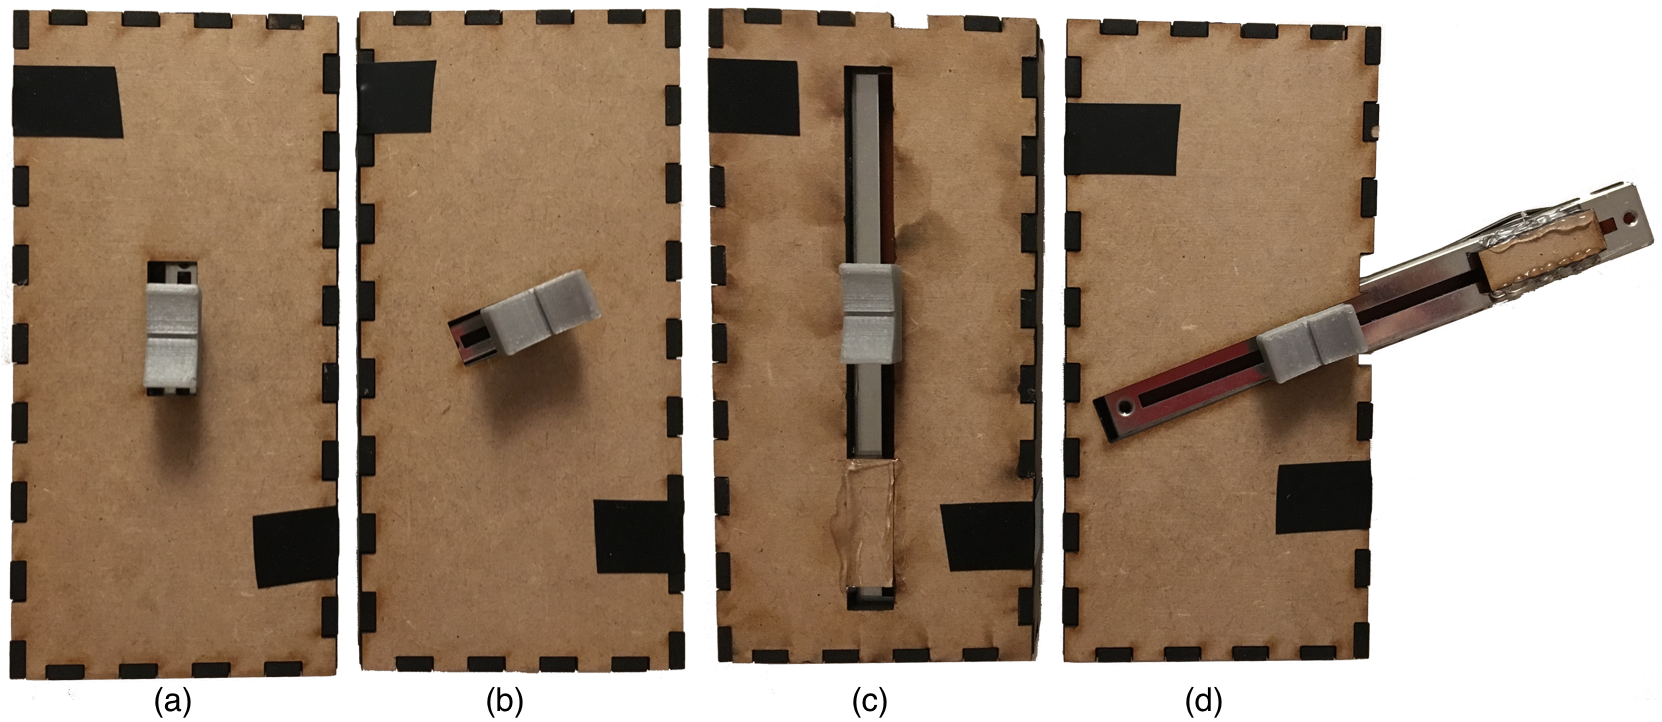
\includegraphics[width=1\columnwidth]{figures/prototypes}
  \caption{(a): small length/vertical orientation slider. (b): small length/tilted orientation slider. (c): large length/vertical orientation slider. (d): large length/tilted orientation slider}
  \label{fig:figure2}
\end{figure}
%================================================

%================================================
\begin{figure}[h]
\centering
  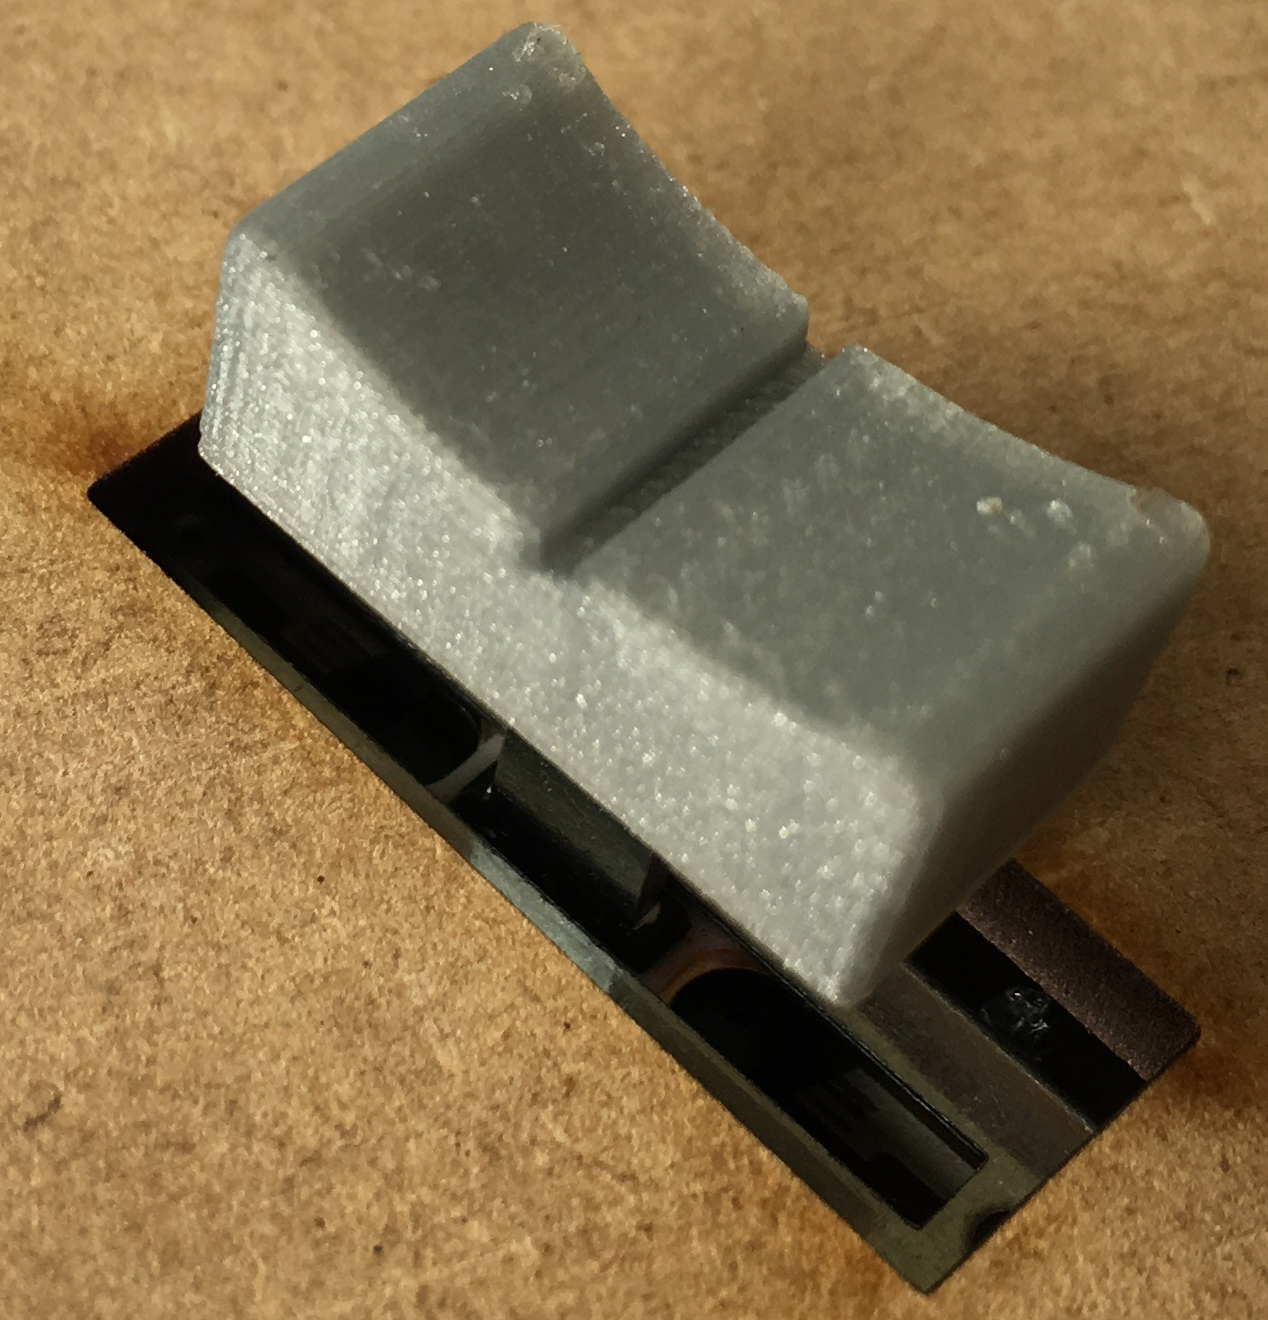
\includegraphics[width=0.4\columnwidth]{figures/knob}
  \caption{Slider's knob shape used on prototypes. The concave shape allows an easier grip for thumb interaction.}
  \label{fig:figure3}
\end{figure}
%================================================

The four prototypes were connected to an Arduino Mega 2560 board in order to make the connection with our pointing software. This software ran the experimental task on a 15 inches MacBook Pro (Retina, Mid 2015) screen with 110 pixels per inch to display the task.

Ten volunteers (22-33 years old, M=27.2, SD=3.1, 3 female) were recruited on campus. All were right-handed and owners of touchscreen phones.

%----------------------------------------------------------------------------------------
\subsection{Task}
%----------------------------------------------------------------------------------------
The study required participants to perform a pointing task as in previous work \cite{Coutrix2015,Casiez08theimpact} as it is a typical task performed on sliders (e.g. reach a specific volume level). The task consists of positioning a cursor (controlled by the user) inside a target area on top of a thin onscreen vertical white slider of 140mm/606px. The target area has an onscreen width of 7mm/31px in order to resemble the area in which slider’s cursor of the video will be positioned. The user’s cursor is a thin horizontal line that the user can control in a vertical way. A visual feedback of the error from the user’s cursor to the target area is displayed along the slider (Figure \ref{fig:figure4}).

%================================================
\begin{figure}[h]
\centering
  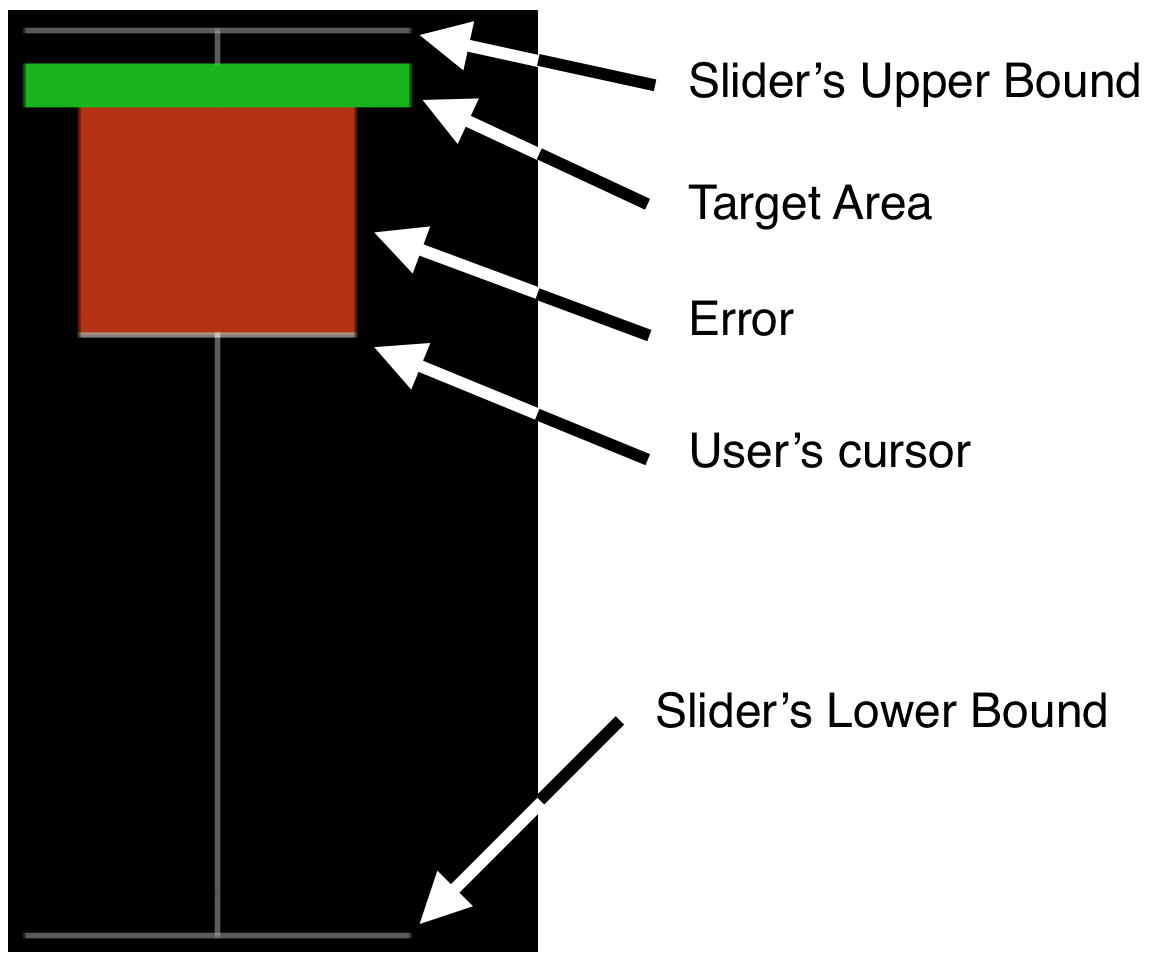
\includegraphics[width=0.7\columnwidth]{figures/slidertask}
  \caption{Screenshot of the experimental pointing task with a slider of 140mm/606px.}
  \label{fig:figure4}
\end{figure}
%================================================

Participants were asked to be as fast and accurate as possible on the pointing task. As in \cite{Coutrix2015}, the error rate is forced to zero. This means that the task must be completed successfully, i.e. the user’s cursor must stay in the target width for 1 second. We chose this validation mechanism to avoid additional actions to confirm the pointing \cite{Zhang:2012:MDE:2212776.2223704} After the task is completed successfully, a new target appears in a predefined distance of 100mm/433px in relation to the location of the user’s cursor.

The target’s width and distance were selected result in a single Fitt’s index of difficulty  (ID) of 4, which is within the ID range used in \cite{Casiez08theimpact}; this value was given by $ID = log2((D/W)+1)$, where \textit{D} is the distance between the user’s cursor position and the target area, and \textit{W} is the target area width. The Control-Display gain difference for both large sliders (CD gain = 2) and small sliders (CD gain = 7) are within the range of the CD gains that do not affect significantly the movement time as computed by Casiez et al. in \cite{Casiez08theimpact}.

%----------------------------------------------------------------------------------------
\subsection{Procedure}
%----------------------------------------------------------------------------------------
At first, participants were introduced to the prototypes and tasks through a training phase. After the training, the trials started. As in Grossman \& Balakrishnan work \cite{Grossman:2005:BCE:1054972.1055012}, the tasks were performed in pseudo-random order through 2 blocks (according to the NH variable) to avoid disturbing the participants with several changes among the grasping conditions. Half of the participants started with the One-handed condition and the other half with the Two-handed condition. Each block was divided in 4 sub-blocks representing the 4 possible combinations from the Length $\times$ Orientation conditions which were presented to the participants in random order; a small break was given to participants after each sub-block. For each sub-block 17 repetitions were performed; the first repetition was used for training. A total of 1280 pointing tasks were collected, by 10 participants $\times$ 16 task repetitions $\times$ 2 Number of Hands $\times$ 2 Lengths $\times$ 2 Orientations (160 measures for each Number of Hands $\times$ Length $\times$ Orientation conditions).

Along the experiment participants were recorded in order to analyse the way how they interacted with the prototypes. The study ended with participants answering a SUS form to evaluate the 4 presented conditions (2 Lengths $\times$ 2 Orientations) for one-hand operation.

%----------------------------------------------------------------------------------------
\section{Results and Discussion}
%----------------------------------------------------------------------------------------
A Shapiro-Wilk test revealed that we could not assume the homogeneity of the data and thus, we analysed our data using a Friedman non-parametric test. The test revealed an impact on the movement time for the slider’s length ($\chi^2$ = 25.6, \textit{p}<0.001) (see Figure \ref{fig:figure5}), we believe that this difference is due to the difficulty of performing the task in a small motor space; the task was too difficult with small sliders and significantly less difficult to perform with larger sliders.

%================================================
\begin{figure}[h]
\centering
  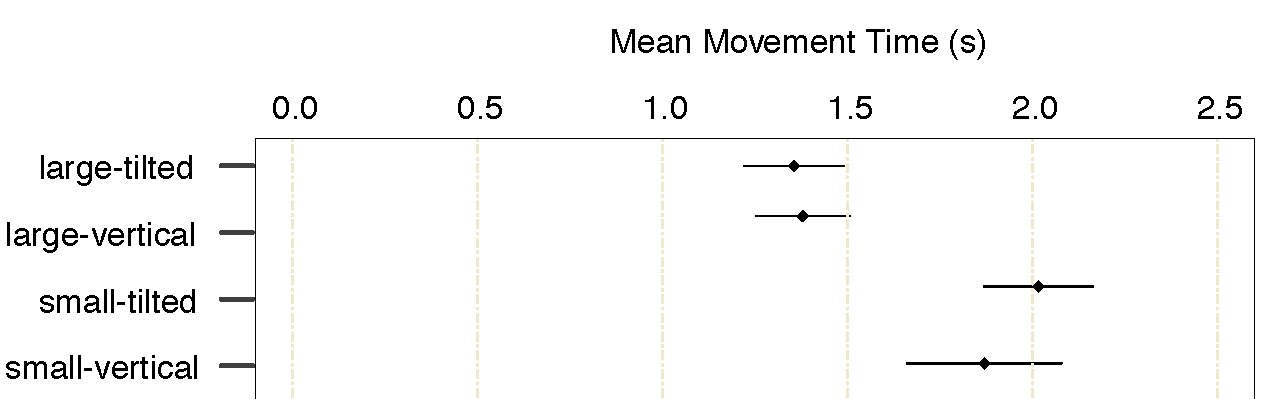
\includegraphics[width=1\columnwidth]{figures/movementTime}
  \caption{Average movement time for the 4 possible: conditions Lengths $\times$ Orientations. (error bars: 95\% confidence interval)}
  \label{fig:figure5}
\end{figure}
%================================================

Post-hoc test using Wilcoxon test with Bonferroni correction showed statistically significant difference between vertical and tilted orientation (\textit{p}<0.03) for small sliders and a marginal statistically significant difference (\textit{p}<0.5) for large sliders.

For small sliders, since both orientations fit within the functional area of the thumb, the results could suggest that flexion-extension movements are more efficient that adduction-abduction movements performed with the thumb (Figure \ref{fig:figure6}), confirming the thumb’s movements results in \cite{Karlson06understandingsingle-handed}. Another factor to highlight is the familiarity of the orientation; some participants commented that they prefer the common vertical orientation because resembles other appliances (e.g. graphic sliders on mobile phones).

Surprisingly, the time difference was marginal between the large sliders. We noticed that all the participants changed the grip of the device in order to allow the thumb to move the vertical slider; on the contrary, all the participants kept the same grip with the tilted slider. This suggest that changing the grip of the device, to reach outside medium difficulty level of the functional area of the thumb, does not have a big impact on the performance.

The SUS test given to participants after the experiment revealed that the large-vertical slider was the most appreciated by the users (Table 1), ranking higher than the rest of the conditions. In despite of this, several participants remarked that the large-tilted slider was more comfortable to use: \textit{“I found the tilted one more suitable with the thumb, because it's in the same direction of the motion”}; \textit{“I’d choose the big tilted one for one-handed task for its better ergonomics”}; \textit{“I liked more the tilted one because it was easier to use with one hand”}; \textit{“For one hand, I found  the large tilted slider easier to manipulate”}.

\begin{table}[h]
\centering
\caption{SUS score for each of the 4 possible conditions}
\label{my-label}
\begin{tabular}{|c|c|c|}
\hline
\textbf{Length} & \multicolumn{1}{l|}{\textbf{Orientation}} & \textbf{SUS score} \\ \hline
Small           & Vertical                                  & 73,75              \\ \hline
Small           & Tilted                                    & 68,75              \\ \hline
Large           & Vertical                                  & 76,875             \\ \hline
Large           & Tilted                                    & 68,75              \\ \hline
\end{tabular}
\end{table}

%----------------------------------------------------------------------------------------
\section{Conclusion and Future Work}
%----------------------------------------------------------------------------------------
In this work we have analysed the impact on performance when reaching medium difficulty level of the functional area of the thumb, by increasing the motor space. We found a significant impact on performance between large and small sliders. The orientation had a significant impact as well on small sliders; on the contrary, for large sliders it was not the case. We found that reaching medium difficulty level of the functional area of the thumb affects marginally the performance in comparison with the easy difficulty level. We want to extend this study by further increasing/decreasing the motor space and analyse the limits for thumb interaction on tangible sliders, before the performance is dramatically compromised.
%----------------------------------------------------------------------------------------
\section{Remerciements}
%----------------------------------------------------------------------------------------
Ce document est bas\'e sur le mod\`ele des soumissions aux conf\'erences SIGCHI, ainsi que sur ceux des conf\'erences IHM pr\'ec\'edentes. Merci \`a leurs nombreux auteurs.

% Balancing columns in a ref list is a bit of a pain because you
% either use a hack like flushend or balance, or manually insert
% a column break.  http://www.tex.ac.uk/cgi-bin/texfaq2html?label=balance
% multicols doesn't work because we're already in two-column mode,
% and flushend isn't awesome, so I choose balance.  See this
% for more info: http://cs.brown.edu/system/software/latex/doc/balance.pdf
%
% Note that in a perfect world balance wants to be in the first
% column of the last page.
%
% If balance doesn't work for you, you can remove that and
% hard-code a column break into the bbl file right before you
% submit:
%
% http://stackoverflow.com/questions/2149854/how-to-manually-equalize-columns-
% in-an-ieee-paper-if-using-bibtex
%
% Or, just remove \balance and give up on balancing the last page.
%
\balance{}

% REFERENCES FORMAT
% References must be the same font size as other body text.
%\bibliographystyle{unsrt}
\bibliographystyle{SIGCHI-Reference-Format}
\bibliography{sample}

\end{document}
%----------------------------------------------------------------------------------------

%%% Local Variables:
%%% mode: latex
%%% TeX-master: t
%%% End:
